% Verbatim source: Report/initial/3b_Neural_Network_full.docx
\addsec{\src{Model and Set-up}}

\src{A feedforward neural network passes the inputs through layers of neurons, each of which-h applies a non-linear activation function, such as the sigmoid, to a weighted sum of its inputs. This non-linearity is what lets the network learn non-linear relationships (Wüthrich \& Merz, 2023, pp. 269-273). We use the R package nnet, which fits networks with a single hidden layer and optimises the weights with the BFGS method (Ripley \& Venables, 2026). Since flexible networks can also fit the noise in the training data, we keep the network small and add weight decay, which can improve generalisation (Krogh \& Hertz, 1992, p. 950). The 13 predictors are rescaled to [0, 1], as inputs on similar scales help the weights learn at a similar rate (LeCun et al., 1998, Sect. 4.3). The minimum and maximum come from the training set only, so that no information from the test set leaks into the model (Kapoor \& Narayanan, 2023, pp. 1-3).}

\addsubsec{\src{Tuning and Threshold Selection}}

\src{We tune the number of hidden neurons (1, 2, 3 or 5) and the weight decay (0.01, 0.1, 0.5 or 1) with the caret package (Kuhn, 2008). As for the random forest, we use 10-fold cross-validation in which all programmes of a country stay in the same fold, because randomly split folds give over-optimistic error estimates and favour overly complex models when observations are dependent (Roberts et al., 2017, p. 914). Models are compared by balanced accuracy, the mean of sensitivity and specificity, because plain accuracy gives an optimistic estimate for a biased classifier on imbalanced data (Brodersen et al., 2010, p. 3121).}

\begin{wordtable}
\centering
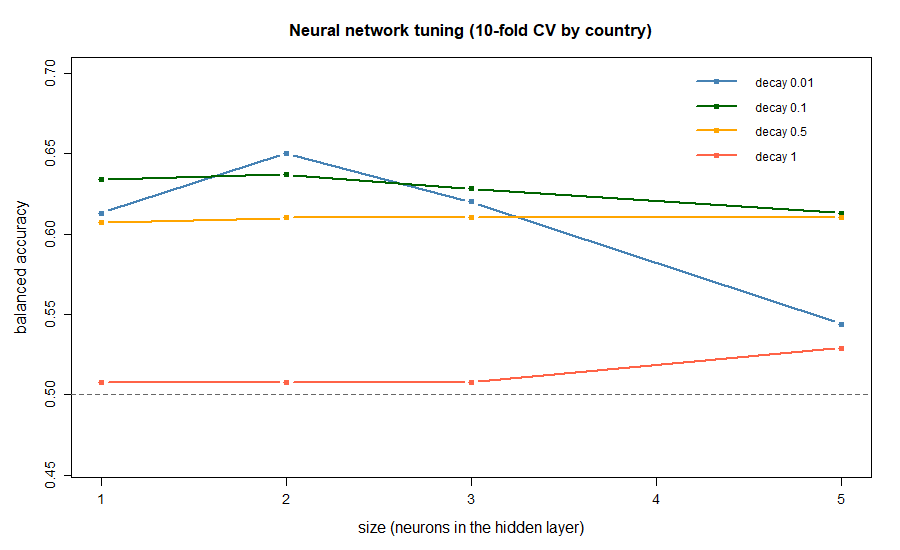
\includegraphics[width=0.94\linewidth]{../Neural_Network/fig_nn_tuning.png}
\wordcaption{\src{\textbf{Figure 1:} Cross-validated balanced accuracy by number of hidden neurons and weight decay (10-fold CV by country, 145 training programmes; dashed line = 0.500).}}
\end{wordtable}

\src{The best network has two hidden neurons and a decay of 0.010, with a cross-validated balanced accuracy of 0.650 (Figure 1). With the same light decay, five neurons only reach 0.544, while a strong decay of 1 keeps every size between 0.510 and 0.530, close to the 0.500 of a model that always predicts the same class. With 145 training programmes, a small and lightly regularised network therefore works best. We then choose the classification threshold that maximises balanced accuracy on the out-of-fold predictions, so that the test set plays no role in model selection. This gives a threshold of 0.440 and an out-of-fold balanced accuracy of 0.684.}

\addsubsec{\src{Test-Set Results and Discussion}}

\src{Table~\ref{tab:model-comparison} compares the final network (13 inputs, 2 hidden neurons, 31 weights) with the group's other models on the 28 test programmes approved between 2014 and 2016. The AUC is the probability that a model ranks a randomly chosen interrupted programme above a randomly chosen completed one, so 0.500 corresponds to random guessing (Fawcett, 2006, p. 867).}

\begin{wordtable}
\wordtablecaption{tab:model-comparison}{\src{\textbf{Table \thetable:} Test-set performance of all models (28 programmes, 2014–2016).}}
\begin{tabularx}{\linewidth}{@{}Xrrrrr@{}}
\toprule
\textbf{\src{Model}} & \textbf{\src{Accuracy}} & \textbf{\src{Sensitivity}} & \textbf{\src{Specificity}} & \textbf{\src{Bal. acc.}} & \textbf{\src{AUC}}\\
\midrule
\src{Neural network} & \src{0.500} & \src{0.294} & \src{0.818} & \src{0.556} & \src{0.567}\\
\src{Random forest (tuned)} & \src{0.500} & \src{0.471} & \src{0.545} & \src{0.508} & \src{0.586}\\
\src{Logistic regression} & \src{0.536} & \src{0.412} & \src{0.727} & \src{0.570} & \src{0.684}\\
\src{Baseline (always interrupted)} & \src{0.607} & \src{1.000} & \src{0.000} & \src{0.500} & \src{0.500}\\
\bottomrule
\end{tabularx}
\end{wordtable}

\src{The network beats the random forest on balanced accuracy (0.556 vs 0.508) but not on AUC (0.567 vs 0.586), and both reach an accuracy of only 0.500, below the 0.607 of predicting an interruption for every programme. The two models also make different errors: the network rarely predicts an interruption (sensitivity 0.294, specificity 0.818), while the forest is more balanced (0.471 and 0.545). The network's result is also fragile. With the default threshold of 0.50 it scores slightly higher on the test set (0.572), and refitting it with 20 different random seeds gives test balanced accuracies between 0.436 and 0.559 (median 0.553). This is expected, since the starting weights are drawn randomly (Wüthrich \& Merz, 2023, p. 284) and the fitted network is not unique.}

\src{We thus find no reliable winner between the two models. With 17 interrupted and 11 completed programmes in the test set, one additional correct prediction moves balanced accuracy by 0.030 to 0.050, as much as the gap between them. The network's balanced accuracy also falls from 0.684 out of fold to 0.556 on the test set, a period in which the share of interrupted programmes rises from 45\% to 61\%. These results are in line with evidence that tree-based models still outperform deep learning on medium-sized tabular datasets of around 10,000 observations (Grinsztajn et al., 2022, p. 507), far more than our 145. Interpretability points the same way: for high-stakes decisions, Rudin (2019) argues for inherently interpretable models over black boxes that are too complicated for humans to comprehend, and the network's 31 weights have no direct economic meaning. Since it brings no clear accuracy gain over the random forest, nor over logistic regression, which has the highest balanced accuracy and AUC in Table~\ref{tab:model-comparison}, we would not use the neural network to flag programmes at risk of interruption.}
